
% 動画は歩きながらあるいは乗り物に乗りながら撮影されることがあり、そうした動画では多くの場合各時点における位置情報がコンテンツにとって重要な意味を持つ
Sometimes a video is recorded with the camera operator walking or riding on a vehicle.
In most cases of that kind of videos, location information at each moments of them have significant meaning in making movie contents.
% 例えば自転車レースを記録した映像であれば、特定の難所を選手が通過するシーンだけを抽出したいといった需要がある
For example, in case of creating a documentary of a bike race, there is a large demand for extracting certain scenes in which riders are passing a dangerous spot.

% 我々は動画に周期的にglobal positionを埋め込むことで編集時に位置情報とタイムスタンプを対応付けられるようにするシステムを開発した
We created a system that embeds geolocation of the camcorder measured by a GPS sensor into a video at intervals of a few seconds.
The path, or the series of geolocations associated with timestamps of a video is used to provide an user interface that enables geolocation-based video editing.
Using this geolocation-based system, user can interact with videos fully exploiting their spatial semantics and without paying extra attention on timestamps in a movie authoring process.

\begin{figure}[htbp]
 \begin{center}
  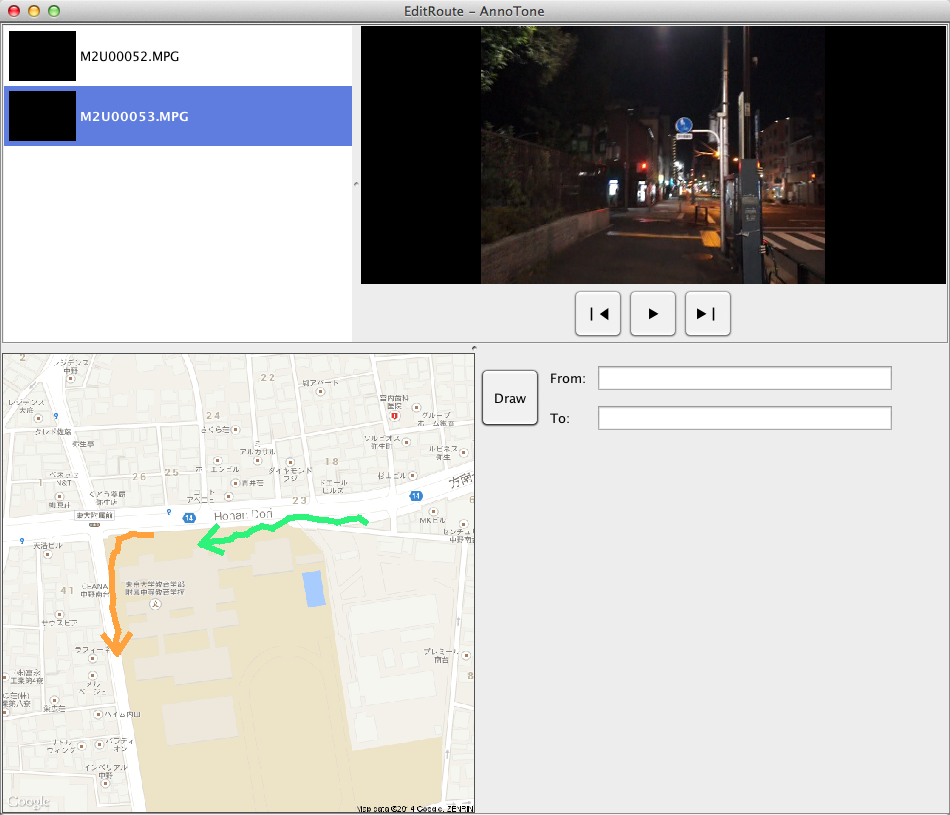
\includegraphics[width=100mm]{application_map.png}
 \end{center}
 \caption{The user interface of our geolocation-based video editor.}
 \label{fig:appl_map}
\end{figure}

% UIの説明
Figure \ref{fig:appl_map} shows the appearance of the interface.
Loaded videos are listed on the upper left listview, and can be watched in the upper right video viewer.
Paths embedded in the videos are visualized in the map below as green and orange winding arrows. That of the currently selected video is colored orange.
User can seek a timestamp of a video at which the camera is in a certain place by double-clicking the corresponding part of the arrow on the map.
If a user double-clicked a curved position of an arrow, the moment of a video at which the camera is turning a corner would be sought.
% クリッピング
User can clip a needed scene from loaded videos by two location-based means in this system.
In the use of first means, a user draws a line that specifies the expected path of the extracted clip along existing paths by his/her hand, then the desired scene is automatically clipped from loaded videos.
On the other hand, the second means only requires its user to specify the names of start and end positions of expected clip, like ``from Paris to London''.
The system automatically finds the geolocations of the two positions using Google Maps API \cite{googlemapsapi} and extracts a section of a video that starts and ends with the specified geolocations.
